
\documentclass[sigconf,authordraft]{acmart}

%%
%% \BibTeX command to typeset BibTeX logo in the docs
\AtBeginDocument{%
  \providecommand\BibTeX{{%
    \normalfont B\kern-0.5em{\scshape i\kern-0.25em b}\kern-0.8em\TeX}}}

%%\setcopyright{acmcopyright}
%%\copyrightyear{2018}
%%\acmYear{2018}
%%\acmDOI{10.1145/1122445.1122456}

%% These commands are for a PROCEEDINGS abstract or paper.
%%\acmConference[Woodstock '18]{Woodstock '18: ACM Symposium on Neural
%%  Gaze Detection}{June 03--05, 2018}{Woodstock, NY}
%%\acmBooktitle{Woodstock '18: ACM Symposium on Neural Gaze Detection,
%%  June 03--05, 2018, Woodstock, NY}
%%\acmPrice{15.00}
%%\acmISBN{978-1-4503-9999-9/18/06}


%%
%% Submission ID.
%% Use this when submitting an article to a sponsored event. You'll
%% receive a unique submission ID from the organizers
%% of the event, and this ID should be used as the parameter to this command.
%%\acmSubmissionID{123-A56-BU3}

%%
%% The majority of ACM publications use numbered citations and
%% references.  The command \citestyle{authoryear} switches to the
%% "author year" style.
%%
%% If you are preparing content for an event
%% sponsored by ACM SIGGRAPH, you must use the "author year" style of
%% citations and references.
%% Uncommenting
%% the next command will enable that style.
%%\citestyle{acmauthoryear}

%%
%% end of the preamble, start of the body of the document source.
\begin{document}

%%
%% The "title" command has an optional parameter,
%% allowing the author to define a "short title" to be used in page headers.
\title{PAVE}

%%
%% The "author" command and its associated commands are used to define
%% the authors and their affiliations.
%% Of note is the shared affiliation of the first two authors, and the
%% "authornote" and "authornotemark" commands
%% used to denote shared contribution to the research.
\author{Samuel Leventhal}
%\authornote{Both authors contributed equally to this research.}
\email{samlev@cs.utah.edu}
\affiliation{%
  \institution{University of Utah School of Computing: Scientific Computing and Imaging Institute}
  %\streetaddress{P.O. Box 1212}
  %\city{Dublin}
  %\state{Ohio}
  %\postcode{43017-6221}
}
%\orcid{1234-5678-9012}
\author{Mark Kim}
\email{kimmb@ornl.gov}
\affiliation{%
  \institution{Oak Ridge National Lab}
  %\streetaddress{P.O. Box 1212}
  %\city{Dublin}
  %\state{Ohio}
  %\postcode{43017-6221}
}

\author{Dave Pugmire}
\authornotemark[1]
\email{pugmire@ornl.gov}
\affiliation{%
  \institution{Oak Ridge National Lab}}


%%
%% By default, the full list of authors will be used in the page
%% headers. Often, this list is too long, and will overlap
%% other information printed in the page headers. This command allows
%% the author to define a more concise list
%% of authors' names for this purpose.
\renewcommand{\shortauthors}{Leventhal and Kim, et al.}

%%
%% The abstract is a short summary of the work to be presented in the
%% article.
\begin{abstract}
  In this work we offer an approachable platform for visualization tasks by employing a neural network for real time rendering and accurate light transport simulation within the framework of Python made compatible for distributed systems and high performance computing (HPC). The provided model is a coalescence of VTK-m, a visualization tookit fit for massively threaded architectures, PyTorch, an  increasingly popular language within machine learning due to robust libraries for neural networks, and Adios, an adaptable unified IO framework for data managment at scale. The resulting work accomplishes this combination by utilizing VTK-m to construct a path trace renderer able to fluidly and efficiently communicate to a conditional Generative Advisarial Network (cGAN) by means of Adios during training. The resulting generative model serves as a filter for rendered images and visual simulations capable of approximating indirect illumination and soft shadows at real-time rates while maintaining quality comparable to offline approaches.
\end{abstract}

%%
%% The code below is generated by the tool at http://dl.acm.org/ccs.cfm.
%% Please copy and paste the code instead of the example below.
%%

 \begin{CCSXML}
<ccs2012>
<concept>
<concept_id>10003752.10003753.10003761.10003762</concept_id>
<concept_desc>Theory of computation~Parallel computing models</concept_desc>
<concept_significance>500</concept_significance>
</concept>
<concept>
<concept_id>10003752.10003753.10003761.10003763</concept_id>
<concept_desc>Theory of computation~Distributed computing models</concept_desc>
<concept_significance>500</concept_significance>
</concept>
<concept>
<concept_id>10003752.10010070.10010071.10010085</concept_id>
<concept_desc>Theory of computation~Structured prediction</concept_desc>
<concept_significance>500</concept_significance>
</concept>
<concept>
<concept_id>10003752.10010070.10010071.10010261.10010276</concept_id>
<concept_desc>Theory of computation~Adversarial learning</concept_desc>
<concept_significance>500</concept_significance>
</concept>
<concept>
<concept_id>10003752.10010070.10010111.10011710</concept_id>
<concept_desc>Theory of computation~Data structures and algorithms for data management</concept_desc>
<concept_significance>500</concept_significance>
</concept>
<concept>
<concept_id>10003752.10003753.10003757</concept_id>
<concept_desc>Theory of computation~Probabilistic computation</concept_desc>
<concept_significance>300</concept_significance>
</concept>
<concept>
<concept_id>10003752.10010070.10010111.10010113</concept_id>
<concept_desc>Theory of computation~Database query languages (principles)</concept_desc>
<concept_significance>300</concept_significance>
</concept>
<concept>
<concept_id>10010405.10010432.10010439.10010440</concept_id>
<concept_desc>Applied computing~Computer-aided design</concept_desc>
<concept_significance>500</concept_significance>
</concept>
</ccs2012>
\end{CCSXML}

\ccsdesc[500]{Theory of computation~Parallel computing models}
\ccsdesc[500]{Theory of computation~Distributed computing models}
\ccsdesc[500]{Theory of computation~Structured prediction}
\ccsdesc[500]{Theory of computation~Adversarial learning}
\ccsdesc[500]{Theory of computation~Data structures and algorithms for data management}
\ccsdesc[300]{Theory of computation~Probabilistic computation}
\ccsdesc[300]{Theory of computation~Database query languages (principles)}
\ccsdesc[500]{Applied computing~Computer-aided design}

%%
%% Keywords. The author(s) should pick words that accurately describe
%% the work being presented. Separate the keywords with commas.
\keywords{VTKm, neural networks, generative adversarial network, Adios, PyTorch, path tracing}

%% A "teaser" image appears between the author and affiliation
%% information and the body of the document, and typically spans the
%% page.
\begin{teaserfigure}
  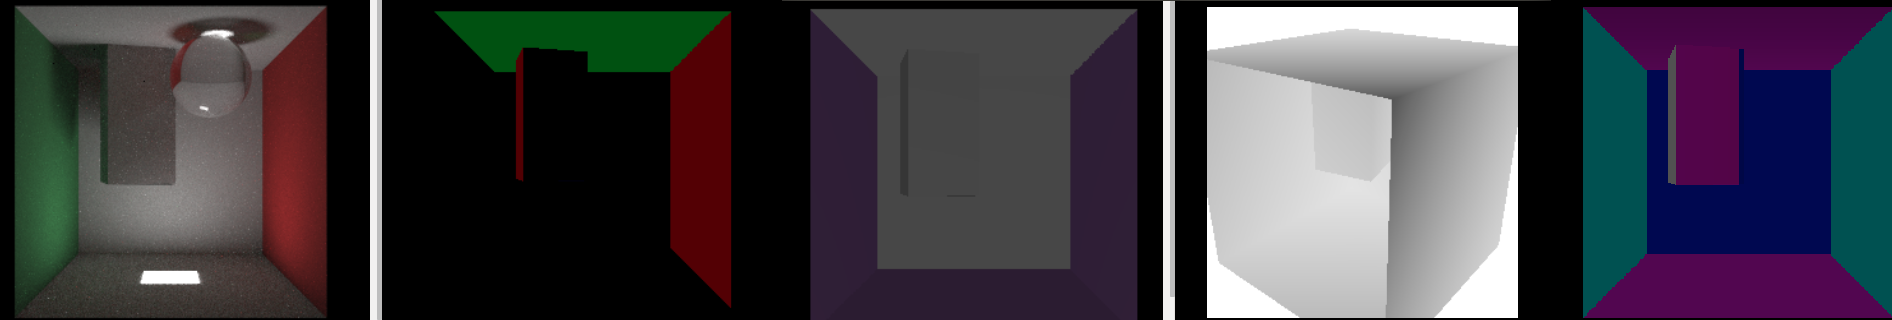
\includegraphics[width=\textwidth]{teaser}
  \caption{Rendered Conditional Images}
  \Description{Conditional Buffers and path traced rendered with VTKm to be used for training a PyTorch conditional generative adversarial network.}
  \label{fig:teaser}
\end{teaserfigure}

%%
%% This command processes the author and affiliation and title
%% information and builds the first part of the formatted document.
\maketitle
\section{Applicable ``Area of Interests'' Targets}
\begin{enumerate}
    \item In situ data management and infrastructures
Current Systems: production quality, research prototypes , Opportunities ,Gaps

Current Systems: integration of VTKm, Adios2 and Python (PyTorch). Prototype being a conditional generative adversarial network (cGAN) designed to use a VTKm based pathtracer applied but not limited to learning global illumination and light behavior in rendering tasks. 
Opportunities: Introducing a framework allowing researchers easy access to python on HPC systems as well as machine learning aided technique to treat and study experimental data used in scientific simulations as learnable probability distributions with derived conditional dependencies of interest.

   \item System resources, hardware, and emerging architectures.
Enabling Hardware, Hardware and architectures that provide opportunities for In situ processing, such as burst buffers, staging computations on I/O nodes, sharing cores within a node for both simulation and in situ processing

Enabling Hardware: By constructing an architecture allowing for Python to interface with VTKm data management controlled by Adios2 the proposed software allows for a well distributed simulation task among cores.

  \item Methods and algorithms:
Analysis: feature detection, statistical methods, temporal methods, geometric and topological methods 
Visualization: information visualization, scientific visualization, time-varying methods
  \item Case Studies and Data Sources
In situ methods/systems applied to data from simulations and/or experiments / observations
  \item Simulation and Workflows:
Integration:data modeling, software-engineering, 
Workflows for supporting complex in situ processing pipelines
  \item Requirements, Usability:
Reproducibility, provenance and metadata

\end{enumerate}

\section{Introduction}


\section{Related Work}

Real time true to life quality rend3erings of light transport remains an active area of research with a number of various approaches such as precomputed radiance transfer, \cite{sloanPrecompRad}

GAN \cite{goodfellowGAN}

cGAN \cite{mirzacGAN}

Tomas and Forbes Deep Illumination: \cite{deepillum}

VTKm \cite{vtkm}

Reinforced learning for light transport simulation \cite{dahmTransport}

\section{Technique Overview}

Utilization of PAVE consists of three consecutive phases: rendering phase of conditional training images, training phase of the generative neural network, and execution phase of the trained network. Three core components, VTK-m, PyTorch, and Adios2 fufill a unique functional requirement during each stage. In this section we describe the independent design and global role each system plays.

\subsection{System Overview}
 
To achieve our goal of a conditional generative neural network capable of rendering geometric dependent object path simulations we begin by rendering informative conditional image buffers along with ground truth scene renderings. For this purpose the VTK-m was chosen due to its scalability and robust capability for HPC visualization tasks. Provided the training set of conditional and ground truth images two neural networks, one convolutional and one generative, play a zero-sum game common to training GANs. To segue data managment of training images the path tracer saves the training set in a distributed setting with the use of Adios2. During training PyTorch is then able to retrieve needed image data through the use of the adaptable IO provided by Adios's Python high-level APIs.

\subsection{Path Tracer Design}

Conditional image attributes and high quality ground truth rendered images are required for the training stage. For this reason the first stage of PAVE consists of generating a visual scene or simulation with VTK-m. Within the framework of VTK-m the implemented ray tracer renders images through means common to commercial ray tracers such as Monte Carlo sampling for shapes of interest, light scattering, randomly directed light paths, material sampling and direct sampling. The image buffers needed to compute light paths afford an informative conditional dependence on the behavior of lighting based on the geometry and light sources within a scene. These conditional buffers, namely albedo, direct lighting, normals of surfaces and depth with respect to camera are then stored within VTK-m with Adios to maintane scalability of the system. For subsequent phases of PAVE the training data can then be retrieved from file again through Adios differing only in the API needed. 

\subsection{Neural Network Design}

The cGAN used closely follows that introduced by Thomas and Forbes with Deep Illumunation \cite{deepillum}. Both the desriminator and generator network are deep convolutional neural networks implemented in PyTorch using training data retrieved from Adios files formated and stored by the VTK-m path tracer. The training stage relies on four conditional buffers depth, albedo, normals and direct lighting along with an associated ground truth image of high light sample count and ray depth. Given the four conditional buffers the generator attempts to construct the ground truth image from noise. The discriminator is then fed both the generated and ground truth image. The loss used for the gradient backpropagation update of both networks is based on the quality of the descriminators ability to classify the artifical and true image in which the generator is greater penalized when the discriminator accurately differentiates the two images, and similarly, the discriminator has a larger loss when incorrectly identifying real from fabricated images. The generator is then considered to have converged when the descriminator predicts both generated and true images with equal probability. 

\subsubsection{Descriminator Network}

For descriminating between artificial and ground truth image renderings a deep convolutional patchGAN network is used motivated by the added advantage of providing a patch-wise probability of an image in question as being real or fake. The benefit of a patch-wise probability allows for higher regional accuracy within an image as well as applicable for image-to-image tasks as introduced by Isola et. al. \cite{isolaPatch}.

\subsubsection{Generator Network}

The generative network used is a deep convolutional network consisting of an encoder and decoder with skip connections concatonating equal depth layers of the encoding and decoding stages. Due to the illustrative `shape' of this design the network is denoted a U-Net as introduced by Ronneberger et. al. for medical segmentation \cite{ronnebergerUnet}. The motivation for utilizing a U-Net is due to success of the skip connections linking the decoded convolutional process to the encoded deconvolutional in capturing geometric and spatial attributes.

\section{Experiments}

\subsection{Cornell Box}
\subsection{Streamline Simulation}

\section{Results}

\includegraphics[scale=.5]{science.jpg}
\section{Conclusions}



%%
%% The acknowledgments section is defined using the "acks" environment
%% (and NOT an unnumbered section). This ensures the proper
%% identification of the section in the article metadata, and the
%% consistent spelling of the heading.
\begin{acks}
Identification of funding sources and other support, and thanks to
individuals and groups that assisted in the research and the
preparation of the work should be included in an acknowledgment
section, which is placed just before the reference section in your
document.
\end{acks}

%%
%% The next two lines define the bibliography style to be used, and
%% the bibliography file.
\bibliographystyle{ACM-Reference-Format}
\bibliography{pave_ref}

%%
%% If your work has an appendix, this is the place to put it.
\appendix

\section{Appendix}



\end{document}
\endinput
%%
%% End of file `sample-authordraft.tex'.
